\documentclass{standalone}
\usepackage{tikz}
\usetikzlibrary{shapes.geometric, arrows.meta, positioning}

\begin{document}
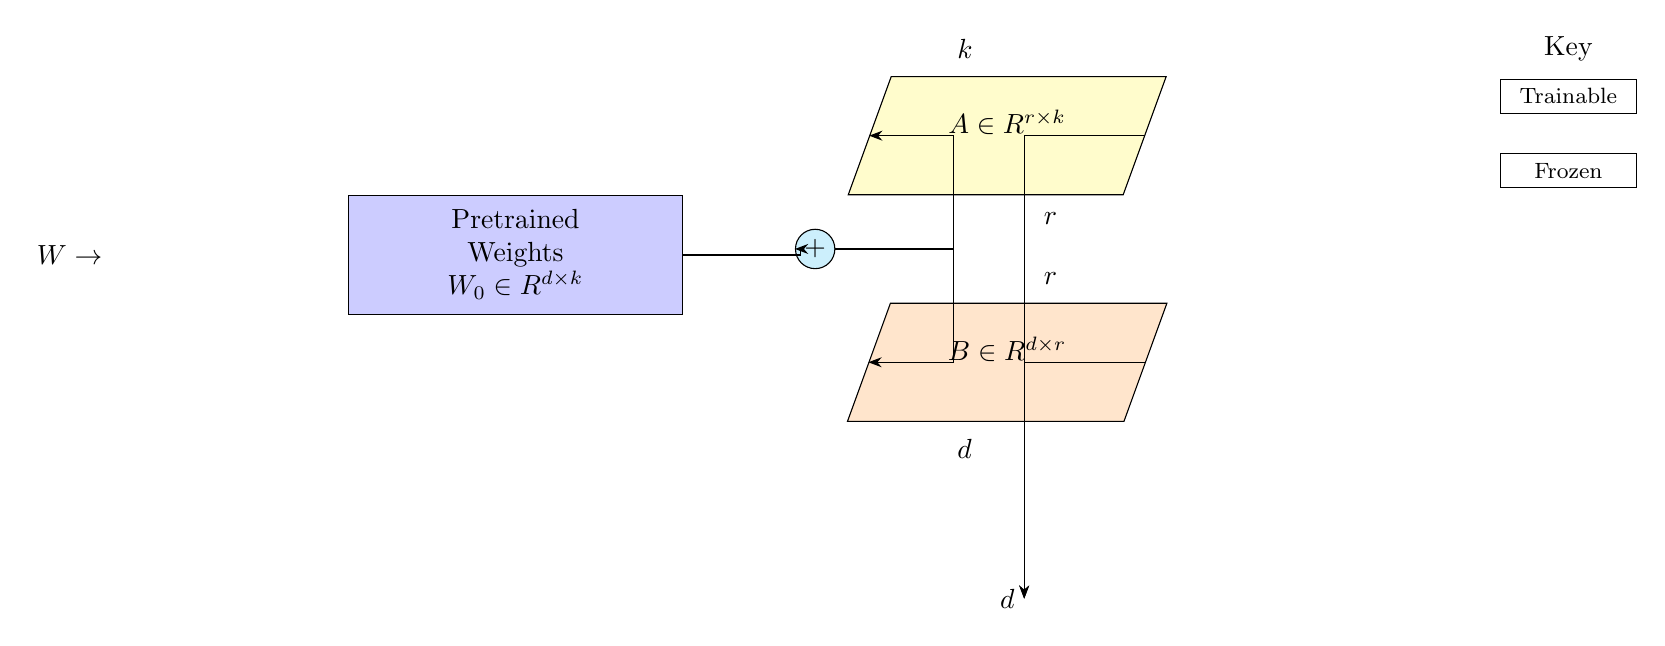
\begin{tikzpicture}[
    node distance = 1.5cm,
    block/.style={rectangle, draw, fill=blue!20, text width=4cm, text centered, minimum height=3em},
    matrix/.style={trapezium, draw, trapezium left angle=70, trapezium right angle=110, align=center, minimum width=3cm, minimum height=1.5cm},
    sum/.style={circle, draw, inner sep=1pt, minimum size=0.5cm, fill=cyan!20},
    key/.style={draw, text width=1.5cm, minimum height=1em, align=center, font=\footnotesize},
    >=Stealth
]

% Draw the Pretrained Weights block
\node[block, fill=blue!20] (weights) {
    \begin{tabular}{c}
        Pretrained \\
        Weights \\
        $W_0 \in \mathbb{R}^{d \times k}$ \\
    \end{tabular}
};

% Draw the addition symbol
\node[sum, right=of weights.north east, anchor=north west, yshift=-0.5cm] (add) {$+$};

% Draw the matrices A and B
\node[matrix, above right=0.5cm and 1.5cm of add, fill=yellow!20] (matrix_A) {
    $A \in \mathbb{R}^{r \times k}$ \\[-0.5ex]
};
\node[matrix, below right=0.5cm and 1.5cm of add, fill=orange!20] (matrix_B) {
    $B \in \mathbb{R}^{d \times r}$ \\[-0.5ex]
};

% Draw the dimensions labels
\node[above=0.1cm of matrix_A.north west, anchor=south west] {$k$};
\node[below=0.1cm of matrix_A.south east, anchor=north east] {$r$};
\node[below=0.1cm of matrix_B.south west, anchor=north west] {$d$};
\node[above=0.1cm of matrix_B.north east, anchor=south east] {$r$};

% Draw the trainable/frozen key
\node[key, right=of matrix_A, xshift=3cm, yshift=0.5cm] (trainable_key) {Trainable};
\node[key, below=0.5cm of trainable_key] (frozen_key) {Frozen};

% Draw the "Key" label
\node[above=0.1cm of trainable_key, anchor=south] {Key};

% Draw the input/output arrow
\node[left=of weights, xshift=-1.5cm] (input_W) {$W \rightarrow$};
\node[below=of matrix_B, yshift=-0.5cm] (output_d) {$d$};

% Draw the connecting lines
\draw[->] (weights.east) -- ++(1.5,0) |- (add.west);
\draw[->] (add.east) -- ++(1.5,0) |- (matrix_A.west);
\draw[->] (add.east) -- ++(1.5,0) |- (matrix_B.west);
\draw[->] (matrix_A.east) -| (output_d.east);
\draw[->] (matrix_B.east) -| (output_d.east);

\end{tikzpicture}
\end{document}